\documentclass[12pt]{ctexart} % 使用 ctexart 文档类支持中文

\usepackage{fancyhdr} % 奇特的 header
\usepackage{xcolor} % 更多颜色

\usepackage[utf8]{inputenc} % 支持 UTF8 字符,在 UTF8 engine 中无需此行
\usepackage{xeCJK} % 支持中文排版,已经包含在 ctexart 中
\usepackage{fontspec} % 字体设置
\usepackage{geometry} % 页面布局
\usepackage{titlesec} % 自定义标题样式
\usepackage{setspace} % 设置行距
\usepackage{microtype} % 更多的微调
\usepackage{tabularx} % 表格支持

\usepackage{float} % Add the float package,支持图片位置固定

\usepackage[colorlinks,linkcolor=black,urlcolor=black]{hyperref} % 超链接支持

\usepackage{tocloft} % 自定义目录样式

\usepackage{graphicx} % 图片设置
\graphicspath{ {./images/} }

% 设置页面布局
\geometry{a4paper, margin=1in}

% 设置行距为 1.25 倍
\setstretch{1.25}

% 设置中文字体
\setCJKmainfont{SimSun}[BoldFont={Microsoft YaHei Bold}] % 设置正文为宋体

\setCJKsansfont{Microsoft YaHei}[BoldFont={Microsoft YaHei Bold}] % 标题等无衬线字体为黑体

% 设置英文字体
\setmainfont{Times New Roman}



% 配置页眉和页脚
\pagestyle{fancy}
\fancyhf{}

\renewcommand{\headrulewidth}{0pt}

\setlength{\headheight}{25.60938pt} % Set the headheight to the required value
\addtolength{\topmargin}{-13.60938pt} % Adjust the topmargin to compensate

% 定义颜色
\definecolor{myblue}{RGB}{152, 220, 222} % 蓝色

% 左侧页眉设置, 页码在页眉外侧
\fancyhead[L]{%
  \colorbox{myblue}{%
    \parbox[t]{1cm}{%
      \textcolor{white}{\thepage}%
    }%
  }%
  \hspace{0.5cm}
  总体设计报告
}

% \fancyhead[L]{\leftmark} % 左页显示章节名

% 页眉横线设置
\renewcommand{\headrulewidth}{0.5pt}
\renewcommand{\headrule}{%
  \hbox to\headwidth{%
    \color{black}\leaders\hrule height \headrulewidth\hfill%
  }%
}

% 页脚页数设置
\renewcommand{\footrulewidth}{0pt}
\fancyfoot[C]{\thepage}

% 设置目录样式
\renewcommand{\cftsecfont}{\bfseries} % 目录中章节标题加粗

\titleformat{\section}
  {\normalfont\Large\bfseries} % 移除 \centering
  {\thesection}{1em}{}


% 超链接设置
\hypersetup{
  colorlinks=true,
  linkcolor=black,
  filecolor=magenta,      
  urlcolor=cyan,
}


\begin{document}

\begin{titlepage}
  \centering % 居中对齐
  % \vspace*{1cm} % 从顶部添加一些垂直间距
  
\includegraphics[width=0.6\textwidth]{zjutitle.jpg} % 插入图片
  
  \vspace{2cm} % 添加垂直间距
  
  {\fontsize{36}{48}\selectfont\CJKfontspec{Microsoft YaHei} 总体设计报告} % 标题
  
  \vspace{2cm} % 添加垂直间距
  
  
\includegraphics[width=0.4\textwidth]{zjulogo.jpg} % 插入图片
  
  \vspace{2cm}
  
  {\Huge\CJKfontspec{Microsoft YaHei} 项目主题: \underline{H5游戏分享平台}} % 项目主题 with underline
  
  \vspace{1cm}

  {\Large\CJKfontspec{Microsoft YaHei} 第 1 小组: \underline{肖一鸣、金谞健、马宇恒、杨仕平、周睿}} % 作者
  
  \vspace{1cm} % 添加垂直间距
  
  {\Large\CJKfontspec{Microsoft YaHei} \today} % 日期

\end{titlepage}

\newpage
\tableofcontents % 自动生成目录
\newpage

\section{体系结构设计}

\subsection{目的}
\subsection{体系结构风格}
\subsubsection{以数据为中心的体系结构}

\subsubsection{调用和返回体系结构}

\subsubsection{面向对象体系结构}

\subsubsection{层次体系结构}

\subsubsection{客户端-服务器架构}

\subsubsection{浏览器-服务器架构}

\subsubsection{事件驱动架构}


\subsection{本次设计采用的体系结构风格}


\subsection{体系结构环境图和原型}

\subsubsection{视图层}
\subsubsection{控制层}
\paragraph{控制器}
\subparagraph{安全模块}
\paragraph{服务层}
\subparagraph{订单管理模块}
\subparagraph{购物车管理模块}
\subparagraph{商家管理模块}
\subparagraph{商品管理模块}
\subparagraph{线上聊天模块}
\subparagraph{用户管理模块}
\subparagraph{商品推荐系统模块}
\subsubsection{模型层}
\paragraph{映射层}
\paragraph{模型层}

\section{服务器端设计}

\subsection{服务器架构}
\subsubsection{业务逻辑层}
\subsubsection{服务层}
\subsubsection{映射层}
\subsubsection{模型层}
\subsection{服务器处理流程}
\subsection{数据库设计}


\section{客户端设计}

\subsection{客户端架构}



\subsubsection{视图层}
\subsection{客户端处理流程}

\section{界面原型}

本项目大量参考 \href{https://itch.io}{itch.io} 、\href{https://www.gcores.com/booom/game_lib}{BOOOM暴造} 等游戏资源分享网站
并专注于游戏资源上传和分享、评分功能,大量简化博客、活动宣传、关注、私聊等社区功能。因此界面原型也大致参考这些网站搭建。就算经验不足,也保证不大幅偏离 “最佳实践”。

以下标明 “参考” 的是参考网站的界面设计,其他的则是我们自己设计的界面原型。

\subsection{登录界面}

使用 UAuth2.0 协议登录,用户可以使用第三方账号(最好是zjuam)登录,因此没必要提供注册界面。

\subsection{主页/游戏探索页}


\subsection{游戏筛选页(参考)}

提供按照某种游戏 tag,比如 `Horror` 标签,或者发布时间、游玩平台进行筛选。后续将直接加到首页,便于筛选。
注意最终交付版本不提供价格/购买功能,因此也没有其筛选项。

\begin{figure}[H]
  \centering
  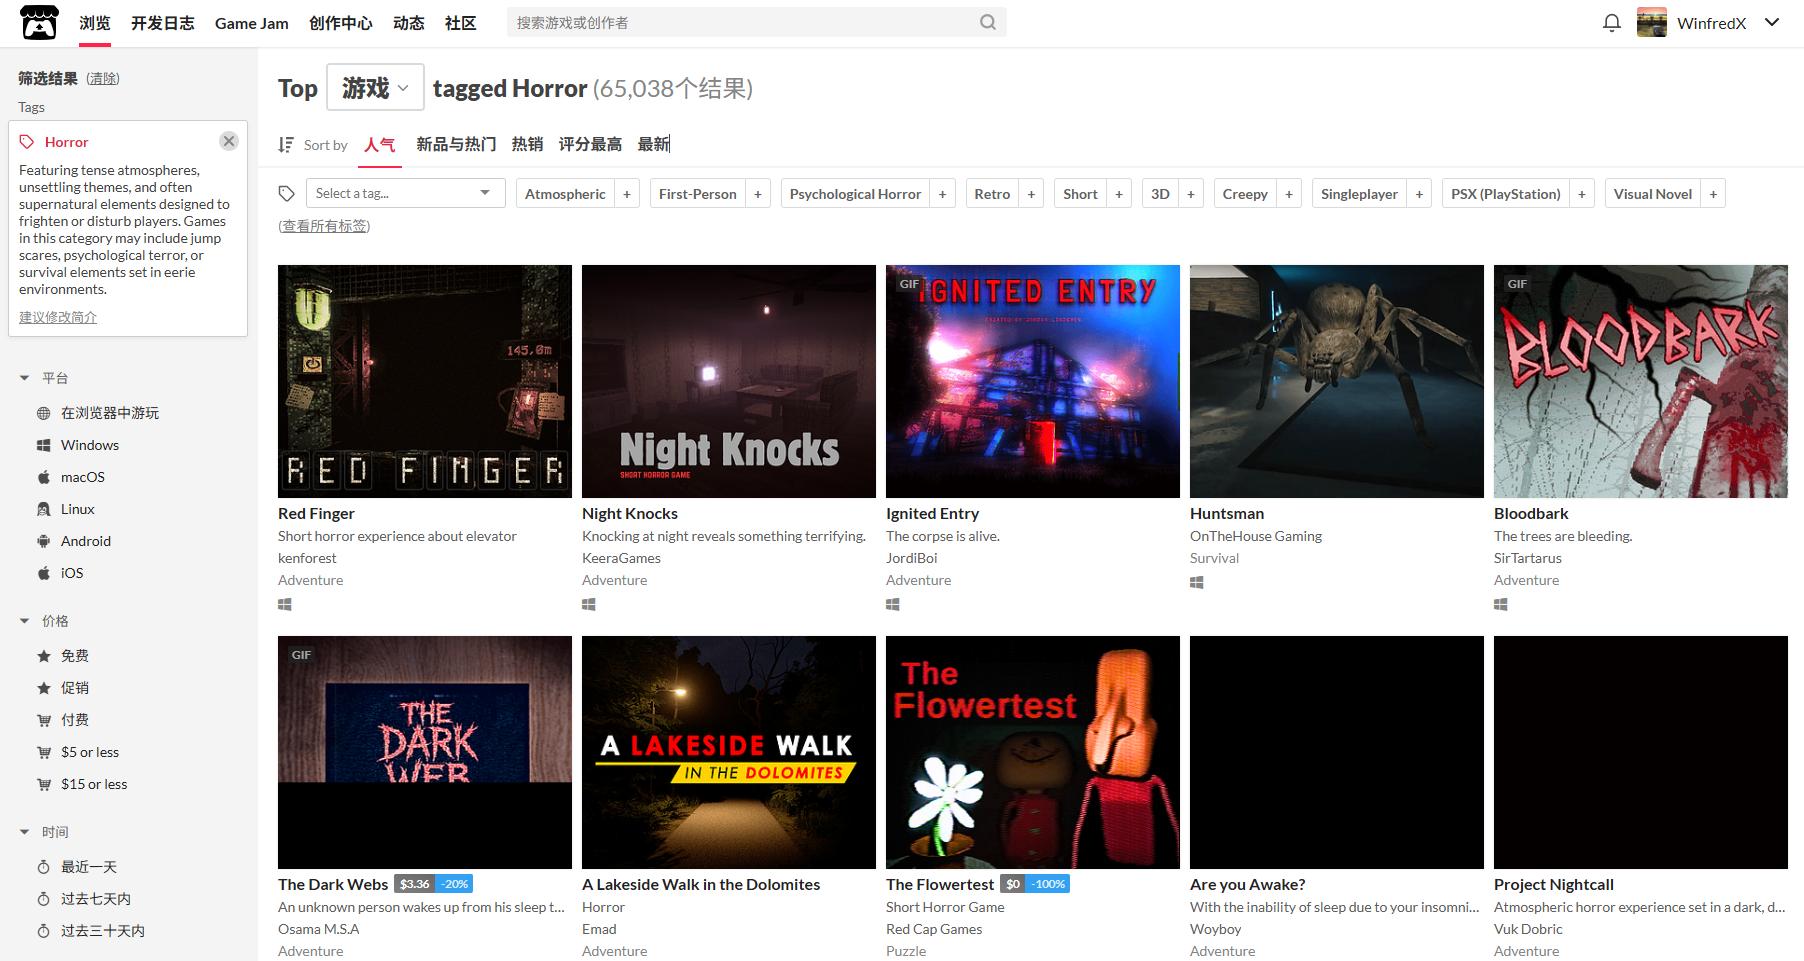
\includegraphics[width=0.8\textwidth]{UI-tagged.png}
  \caption{游戏探索页-按标签筛选}
\end{figure}

\subsection{游戏上传/编辑管理页}

重复利用该表单以实现游戏的上传和所有者/管理员的编辑功能。用户可以在该表单中上传游戏资源,填写游戏信息。


\subsection{游戏详情与进行页}

主要分为纵向两部分,第一个是游玩通道与详细信息,目前已经实现其设计,如果是在线游戏,那么最上方嵌入画布:

\begin{figure}[H]
  \centering
  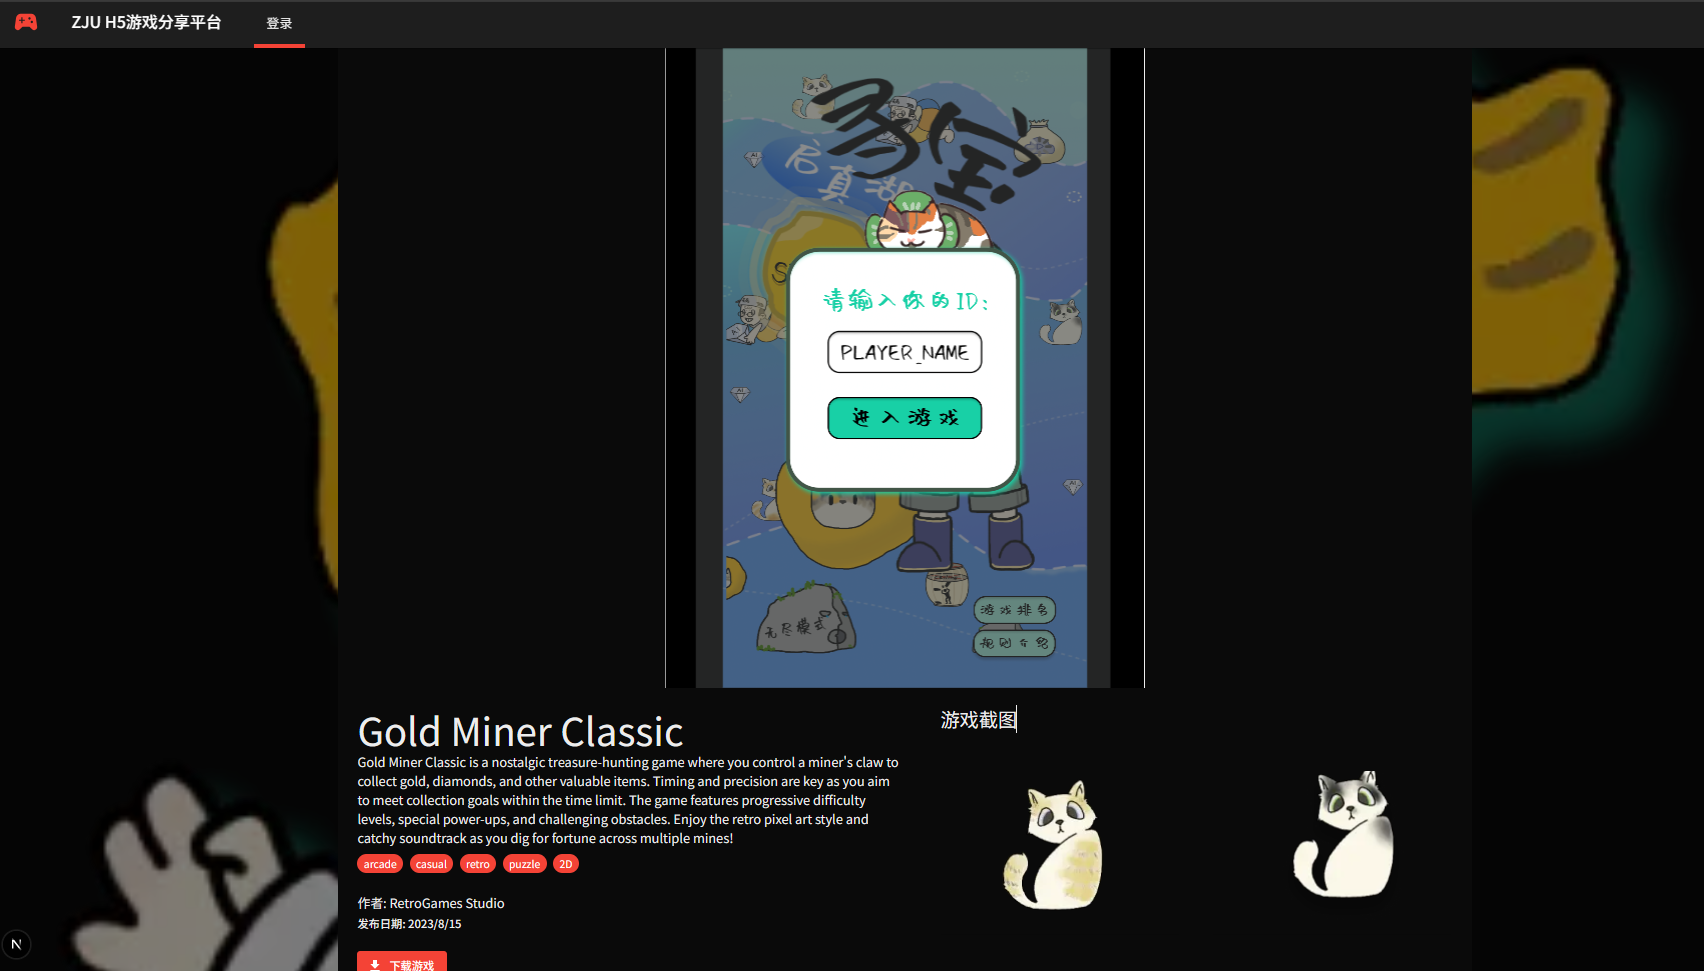
\includegraphics[width=0.8\textwidth]{UI-detailed.png}
  \caption{游戏详情页的游玩和介绍区}
\end{figure}


第二个是打分与评论区,评论区是 itch 网站参考图:


\begin{figure}[H]
  \centering
  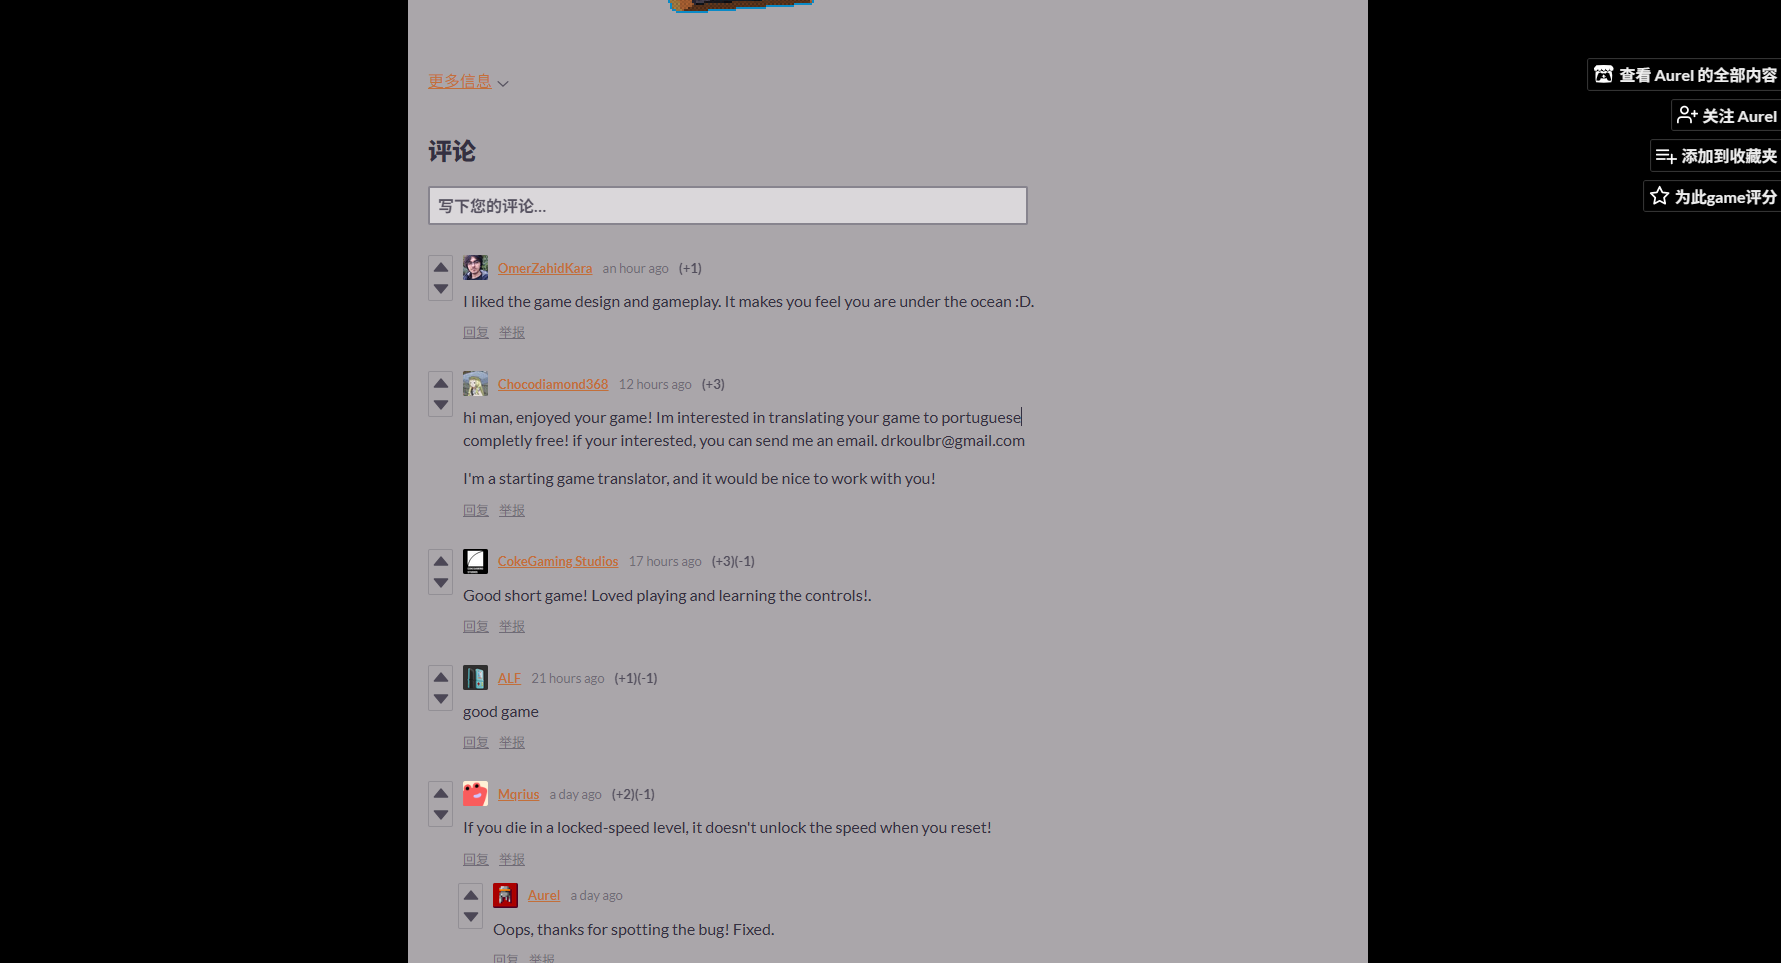
\includegraphics[width=0.8\textwidth]{UI-comment.png}
  \caption{游戏详情页的评论区}
\end{figure}

\subsection{个人信息页(参考)}

在 itch.io 这样创意性十足的网页中,个人信息页是可以灵活编辑其排版和显示内容,甚至可以手动插入 CSS 样式。
但最核心的功能还是个人联系方式和游戏制作列表的展示,简易版将在后续实现。

\begin{figure}[H]
  \centering
  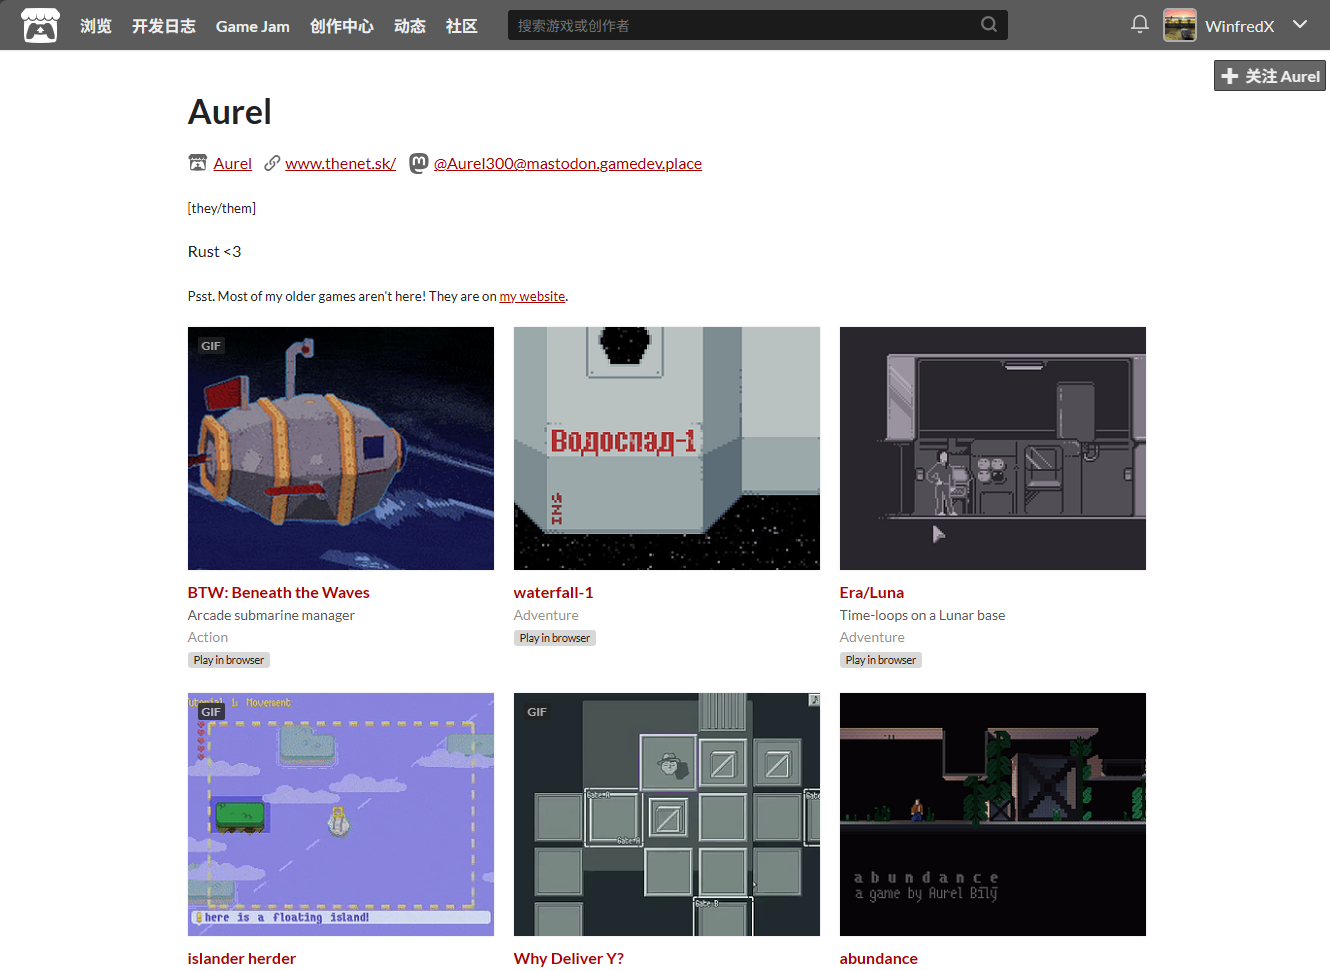
\includegraphics[width=0.8\textwidth]{UI-profile.png}
  \caption{itch.io 的个人信息页}
\end{figure}


\subsection{管理员后台}


\end{document}